\section{Training Methodology}

\subsection{Transforming and Enhancing Data}
In our final runs, the images in the input data are resized to $768 \times 768$.
This size presents a good balance between model performance and training speed: the final results of the models were almost identical to using the entire size of $2048 \times 1024$.
Additionally, this new size makes it possible to use pretrained Swin2 in the entire data instead of having to separate the images of stretch it separately.

The loss of the final mask is calculated on the small, resized image.
When evaluating, the final mask is stretched to its original larger size.

Additionally, we experimented with creating random transforms of the input data, including random flips and random crops.

In different experiments these transforms either replaced or augmented the original training data.
However, this is not present in the final models as their results weren't conclusive: since the original data is complete enough, adding these transforms only made the results on the validation set worse.

\subsection{Loss function}

The choice of loss function is crucial for the performance of our model.

In this assessment, we experimented with three different loss functions.

\begin{description}[style=nextline]
	\item[Categorical Cross-Entropy Loss] All pixels (except the ones marked as background) are equally weighted.
	\item[Intersection over Union Loss] A differentiable version of IoU score, which should ideally work to maximise it.
	\item[Dice Loss] Categories that appear less often are weighted higher\cite{dice_loss}.
\end{description}

Using \textbf{Categorical Cross-Entropy} provided better results in the relevant metrics, including IoU score, when compared to both dice loss and IoU loss.

This surprising result, which can be seen in \cref{iou_vs_cce}, is likely due to the difference in depth of the loss functions.
Since it contradicts some existing literature\cite{dice_loss}, it warrants more exploration later.


\subsection{Optimiser and other Hyperparameters}

There are many possible hyperparameters to enhance the model.


\begin{figure}
	\centering
	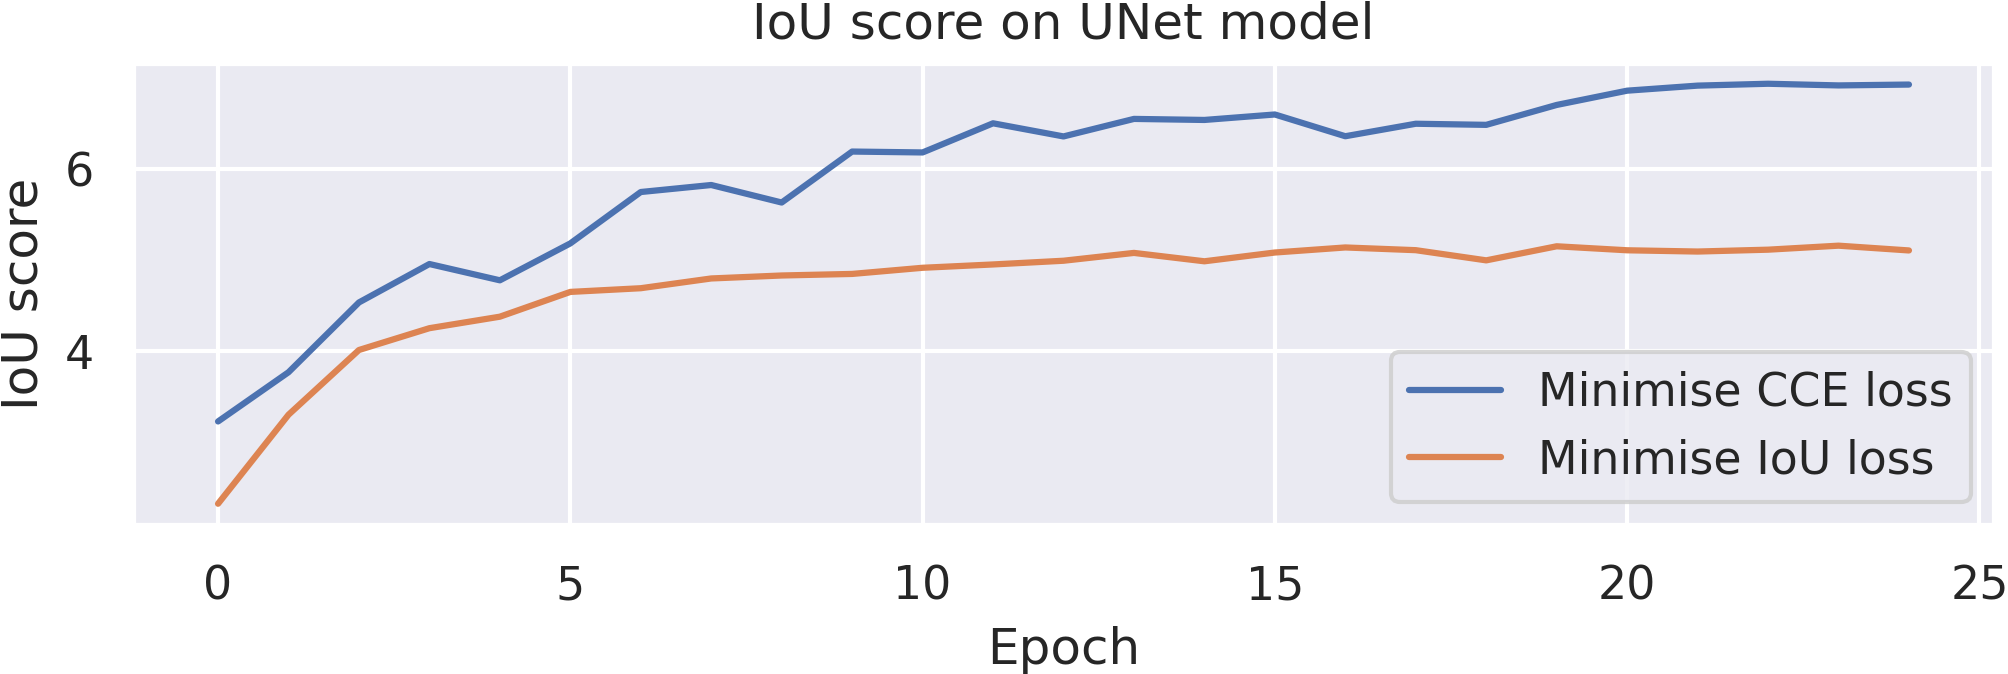
\includegraphics[width=\textwidth]{cce_vs_iou_loss.png}
	\caption{IoU score for UNet models trained to minimise both categorical cross-entropy and a related IoU loss. Surprisingly, the one that optimises CCE has better results.}
	\label{iou_vs_cce}
\end{figure}

\begin{description}[style=nextline]
	\item[Loss Function]
	\item[Optimiser]
		Which optimiser to use to manage the gradient 
\end{description}

